\subsection{Diseño del Resonador}
\label{sss:rr_design}

Para el diseño del simulador, se siguieron los lineamientos descritos en \cite{Lumerical2009}
tanto para el filtro AddDrop como para el filtro Notch. El primero consiste en
el modelo explicado en la sección \ref{ss:generic_theory} con la salvedad que 
la región de Acoplamiento 1 es idéntica a la región de Acoplamiento 2, por lo tanto
$\kappa = \kappa_1 = \kappa_2$, 
$\kappa^* = \kappa_1^* = \kappa_2^*$, 
$t=t_1 = t_2$ y 
$t^*=t_1^* = t_2^*$. 
Adicionalmente, se asume que no hay pérdidas $(\alpha=1)$ y
se seleccionan las características dadas en la tabla \ref{tb:lum_params}.

\begin{table}
\centering
\begin{tabular}{|l|l|}
\hline
Parámetro & Valor \\
\hline
Rango de frecuencias & 1500nm a 1600nm \\ 
$\lambda_0$ & 1550nm \\
Espaciamiento de canales & 200Ghz ó 1.6nm a 1550nm \\
$FSR$ & 3200GHz ó 25.6nm a 1550nm ó 16 canales \\
$\Delta \lambda_{FWHM}$ & 100GHz ó 0.8nm \\
$Q$ & $\frac{1550nm}{0.8nm} \approx 2000$  (\ref{eq:q})\\
\hline
\end{tabular}
\caption{Configuración deseada para el filtro}
\label{tb:lum_params}
\end{table} 

\subsubsection{Índice de grupo $n_g$}

Se calcula el índice de grupo $n_g$ mediante la herramienta MODE de lumérical
(seccion \ref{ss:lumerical}) para encontrar los valores propios en un rango de 
frecuencias de interés. En la gráfica \ref{fig:ng} se
ve el perfil del primer modo a la izquierda y la gráfica de longtud de onda
vs índice de grupo a la izquierda. A partir de ésta, se visualiza que para
$\lambda_0=1550nm$ se tiene $n_g\approx4.8$.

\begin{figure}[h!]
\caption{Índice de grupo. Fuente\cite{Lumerical2009}}
\centering
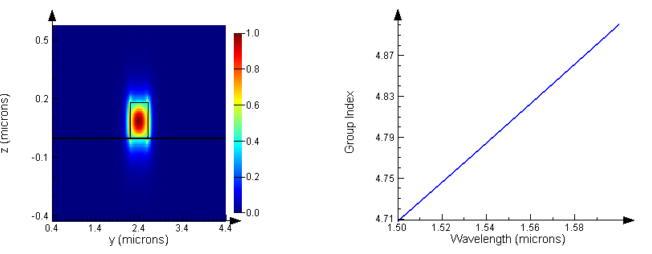
\includegraphics[width=0.8\textwidth,natwidth=652,natheight=254]{figs/ng.png}
\label{fig:ng}
\end{figure} 

\subsubsection{Perímetro del anillo}

Despejando $L$ partir de (\ref{eq:fsr}) y sustituyendo los parámetros 
(Tabla \ref{tb:lum_params}), se tiene:

\begin{align*}
L=\frac{\lambda_0^2}{n_g FSR} 
&=\frac{1550e-9}{4.8 \times 25.6e-9}
 =19.5e-6  \\ %\label{eq:lum_l} \\
R &= \frac{L}{2 \pi} = 3.1 %\label{eq:lum_r}
\end{align*}

\subsubsection{Coeficiente de transmisión y acoplamiento} 

Al despejar $|t_1|$ de (\ref{eq:q}) se tiene:

\begin{equation}
|t|=\sqrt{ \left( \frac{n_g L \pi}{2 Q \lambda} \right) ^2 + 1} - 
    \frac{n_g L \pi}{2 Q \lambda}
\label{eq:t}
\end{equation} 

Y remplazando la configuración dada en la tabla \ref{tb:lum_params}:
\begin{equation*}
|t|=\sqrt{ \left( \frac{4.8 19.5e-6 \pi}{2 2000 1550e-9} \right) ^2 + 1} - 
    \frac{4.8 19.5e-6 \pi}{2 2000 \lambda}
   \approx 0.954
\label{eq:lum_t}
\end{equation*}

El valor de $\kappa$ se obtiene despejando (\ref{eq:eq:energy_conserv}):

\begin{equation}
|\kappa|=\sqrt{1 - |t|^2} \approx 0.301
\label{eq:lum_k}
\end{equation} 


